
\documentclass[master]{thesis-uestc}
\usepackage{listings} 
\lstset{language=C,
   keywords={break,case,catch,continue,else,elseif,end,for,function,
      global,if,otherwise,persistent,return,switch,try,while},
   basicstyle=\ttfamily,
   commentstyle=\color{red},
   stringstyle=\color{dkgreen},
   numbers=left,
   keywordstyle= \color{blue},
   numberstyle=\tiny\color{gray},
   stepnumber=1,
   numbersep=10pt,
   backgroundcolor=\color{white},
   tabsize=4,
   showspaces=false,
   showstringspaces=false}

\title{``支付宝集五福"抽卡概率问题分析}
\author{None}
\advisor{None}
\school{None}
\major{None}
\studentid{None}

\begin{document}

\makecover

\begin{chineseabstract}
    

    2019春节前夕,支付宝如往年一样举办“集五福”活动,在参与的过程中我产生对该问题研究的兴趣,我希望能计算集齐全部5种卡片所需次数的数学期望,以及限制抽取次数能够集齐的概率。
    
    即给定$N$种卡片,每种卡片都有一定的概率$p_i$能被抽到且能被多次抽到。
    
    1. 求恰好集齐时抽取次数的数学期望。

    2. 限制最多抽$M$次,求能够集齐的概率。

    该问题即计算多重集合卡片抽取的期望与限制次数下的概率。本文从该问题出发,研究多种解法,包括蒙特卡洛解法、斯特林数解法,动态规划解法与转化为生成函数后的快速傅里叶变换解法,并比较其复杂度与精确度。

\chinesekeyword{多重集合抽卡概率,蒙特·卡罗方法,状态压缩,概率,动态规划,第二类斯特林数,指数生成函数,快速傅里叶变换}
\end{chineseabstract}

\thesistableofcontents

\thesischapterexordium

\section{研究问题的背景}

本问题来源于生活。2019春节前夕,支付宝如往年一样举办“集五福”活动\footnote{描述:目标是集齐 5 张福卡:“爱国福”、“富强福”、“友善福”、“和谐福”、“敬业福”。有若干次的抽取机会,每次抽取你都有一定概率抽到五张福卡中的一张或抽空,需要在规定次数内集齐五种卡片。},在参与的过程中,运气极差的我依然没有在规定的次数内集齐五张卡片,于是我萌生了计算抽取成功概率的想法。

假设五张卡片的概率是不变的,我希望以五张卡片的概率为输入变量,求解集齐卡片的抽取次数期望。在对问题的建模与思考后,我思考出状态压缩下的动态规划解法后,将其作为2019年3月的南开大学ACM校队选拔赛网络赛的题目\footnote{题目链接:\url{http://acm.nankai.edu.cn/problem/1027}}之一。

但本篇论文不仅仅是该题原题,我在原有问题的基础上进行了修改与条件限制,并提出其它解法,同时将各算法进行对比。


% 计算电磁学方法\citing{wang1999sanwei, liuxf2006, zhu1973wulixue, chen2001hao, gu2012lao, feng997he}从时、频域角度划分可以分为频域方法与时域方法两大类。频域方法的研究开展较早,目前应用广泛的包括:矩量法(MOM)\citing{xiao2012yi,zhong1994zhong}及其快速算法多层快速多极子(MLFMA)\citing{clerc2010discrete}方法、有限元(FEM)\citing{wang1999sanwei,zhu1973wulixue}方法、自适应积分(AIM)\citing{gu2012lao}方法等,这些方法是目前计算电磁学商用软件
% \footnote{脚注序号“\ding{172},……,\ding{180}”的字体是“正文”,不是“上标”,序号与脚注内容文字之间空1个半角字符,脚注的段落格式为:单倍行距,段前空0磅,段后空0磅,悬挂缩进1.5字符;中文用宋体,字号为小五号,英文和数字用Times New Roman字体,字号为9磅;中英文混排时,所有标点符号(例如逗号“,”、括号“()”等)一律使用中文输入状态下的标点符号,但小数点采用英文状态下的样式“.”。}
% (例如:FEKO、Ansys 等)的核心算法。由文献\cite{feng997he,clerc2010discrete,xiao2012yi}可知

\section{研究问题的意义}

本问题在生活中出现广泛,除了支付宝“集五福”活动,诸多游戏的抽卡、宝箱机制均有类似的应用场景。

\section{本文应用的主要算法}

本文应用的主要算法包括蒙特卡洛方法、第二类斯特林数的计算、状态压缩下的动态规划、快速傅里叶变换等。


\chapter{问题建模}

\section{问题建模}

给定n种互不相同的卡片,与数组$P=\{p_1,p_2,p_3,...p_n\}$,进行若干次抽取实验,对于每次实验,卡片$i$被抽中的概率均为$p_i$。($0< \sum\limits_{i=1}^{i=n}{p_i}\leq 1$)
\vspace{0.5cm}

求解:

\begin{enumerate}
\item 若每种卡片可被无限次抽取,不限制抽取次数,求能够恰好抽取全部种类卡片的抽取次数期望。记为问题一。
\item 若每种卡片可被无限次抽取,且限制抽取$m$次,求在m次内(包括m次)全部种类的卡片均被抽到的概率。记为问题二。
% \item 若卡片的抽取次数有限制,记为$A=\{a_1,a_2,a_3...a_n\}$,其中第$i$个卡片最多被命中$a_i$次,限制抽取$m$次,求全部卡片均有被命中的概率。记为问题三。
% \item 若卡片的抽取次数有限制,记为$A=\{a_1,a_2,a_3...a_n\}$,其中第$i$个卡片最多被命中$a_i$次,不限制抽取次数,求能够恰好抽取全部卡片的抽取次数期望。记为问题四。
\end{enumerate}



\section{符号表示}
\begin{table}[!htbp]
    \centering
    \begin{tabular}{c l}
        \hline
        符号 & 描述 \\
        \hline \hline
        $n$ & 卡片的数量\\
        \hline
        $p_i$ & 第$i$种卡片被抽到的概率\\
        \hline
        $m$ & 限制抽取的次数\\
        \hline

    \end{tabular}
    \caption*{符号表示}
    \label{tab:my_label1}
\end{table}

\chapter{蒙特·卡罗方法}
\section{蒙特·卡洛方法介绍}
蒙特卡罗方法$^{[1]}$也称统计模拟方法,是1940年代中期由于科学技术的发展和电子计算机的发明,而提出的一种以概率统计理论为指导的数值计算方法。是指使用随机数(或更常见的伪随机数)来解决很多计算问题的方法。 

20世纪40年代,在冯·诺伊曼,斯塔尼斯拉夫·乌拉姆和尼古拉斯·梅特罗波利斯在洛斯阿拉莫斯国家实验室为核武器计划工作时,发明了蒙特卡罗方法。因为乌拉姆的叔叔经常在摩纳哥的蒙特卡洛赌场输钱得名,而蒙特卡罗方法正是以概率为基础的方法。 

% \section{时域积分方程时间步进算法阻抗矩阵的存储}
% 时域阻抗元素的存储技术也是时间步进算法并行化的关键技术之一,采用合适的阻抗元素存储方式可以很大的提高并行时间步进算法的计算效率。

\subsection{算法分析}

蒙特·卡洛算法利用计算机生成一个随机数的特性,模拟实际抽取卡片的随机过程。对于每次实验,计算机都需要模拟出本次命中的是哪种卡片,直到满足结束条件。

我们利用蒙特卡洛算法作为研究问题的暴力解法,同时也作为答案的一种可信解法。

\subsection{实现过程}

记总实验次数为T。

\begin{enumerate}
    \item 按照概率随机选择一个卡片,该卡片数加一
    \item 重复过程一,直到满足结束条件。
    \item 进行下一次实验
\end{enumerate}


\begin{figure}[!htbp]
    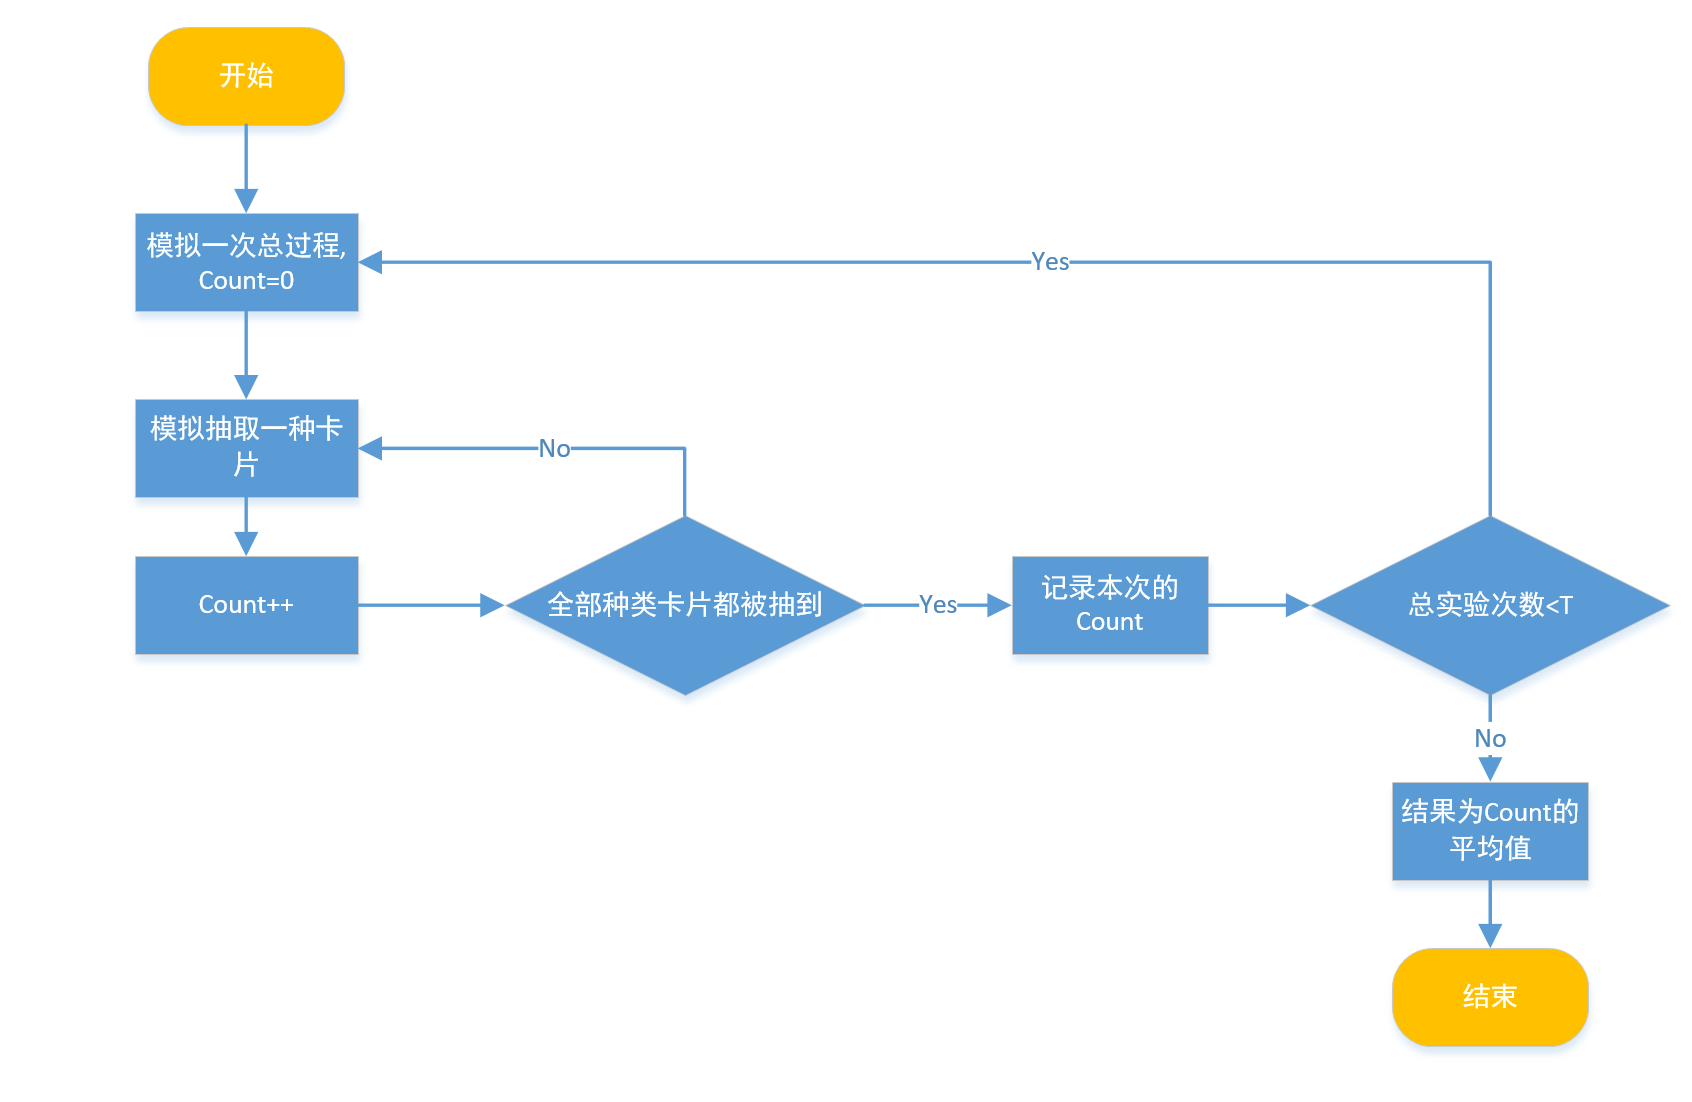
\includegraphics[scale = 0.65]{pic/01.png}
    \caption{问题一:蒙特卡洛算法流程图}
    \label{13214}
    \end{figure}
    

按照概率的选择卡片的方法可优化至$O(logN)$:
    
将卡片对应的概率分布映射到[0,1]的一维区间上,通过生成$[0,1]$的随机数,从而确定对应的卡片。记第$i$张卡片区间为$[\sum\limits_{k=1}^{i-1}{p_k},\sum\limits_{k=1}^{i}{p_k}]$

生成一个随机数$x$后,利用二分查找可以得到随机数$x$对应的区间,复杂度$O(logN)$。

复杂度为O(TElogN),其中$E$为抽取次数期望。

对这个问题来说,蒙特卡洛算法实际上是一种暴力解法,不妨以此解法的答案作为下列解法正确性的标准。

\section{伪代码}

对于问题一,计算期望的蒙特卡洛伪代码如下:

\begin{algorithm}[H]
%  \KwData{this text}
%  \KwResult{how to write algorithm with \LaTeX2e }
 initialization\;
 \While{iteration<T}{
  count=0\;
%   \eIf{understand}{
%    go to next section\;
%    current section becomes this one\;
%    }{
%    go back to the beginning of current section\;
%   }
    \While{Not all the cards were collected}{
        count++\;
        rand=random[0.0,1.0]\;
        i=lower\_bound(prefix\_p,rand) \;
        set card i collected\;
    }
    ans+=count/T\;
 }
 \caption{问题一:蒙特卡洛算法流程}
\end{algorithm}

预处理时,用$prefix\_p$数组存储卡片概率的前缀和,以便在生成随机数进行二分。在判断卡片是否集齐时,可采用将卡片状态转换为一个$N$位二进制数,若第$i$卡片抽到了,则将二进制的第$i$位置为1,如此可$O(1)$判断卡片是否集齐。

对于问题二,限制抽取次数小于等于$M$时集齐的概率,伪代码如下:


\begin{algorithm}[H]
    %  \KwData{this text}
    %  \KwResult{how to write algorithm with \LaTeX2e }
     initialization\;
     \While{iteration<T}{
      count=0\;
        \While{count $\leq$ M and Not all the cards were collected}{
            count++\;
            rand=random[0.0,1.0]\;
            i=lower\_bound(prefix\_p,rand) \;
            set card i collected\;
        }
        \eIf{count$\leq$M}{
            Got++\;
        }{
            Nothing\;
        }
     }
     ans=Got/T\;
     \caption{问题二:蒙特卡洛算法流程}
    \end{algorithm}

\chapter{问题一:期望的计算}

\section{问题分析}

定义刚好抽到$N$张卡片的次数是$X$,设其为事件 $A$,则 $A$ 满足前 X-1 次抽取到的卡片属于某$N$-1种卡片的集合,而第 X 次刚好抽到剩下的第N种卡片。

设$P_X$为X次恰好集齐的概率,则期望为:

$$
E(X)=\sum\limits_{X=1}^{\infty}X*P_X 
$$

根据上述期望公式,若不进行蒙特卡洛随机模拟,似乎必须将$X
$的所有情况全部计算一遍,才能得到一个准确的答案。但这里可以凭借期望可累加的性质和状态转移的思想,利用动态规划求解出一个准确值。

\section{从特殊到一般:卡片概率相同的特殊情况}

先考虑一种比较特殊的情况,卡片概率均相同的特殊情况,即每张卡片的抽取概率都是$\frac{1}{n}$。

接下来存储每个状态,记状态$s(x)$为当前已经抽取了x种卡片,记$dp[x]$为当前处于状态$s(x)$时,抽完剩下$n-x$种卡片所需要次数的期望。

在当前已抽取了x张卡片的情况下,下一次抽取到的是当前已抽取的卡片种类的事件记为A,下一次抽取为剩下的$n-x$种张卡片的事件记为B,则

$$
\begin{array}{lll}

P(A) & = \frac{x}{n} \\
P(B) & = \frac{n-x}{n} \\

\end{array}
$$

则本次实验服从几何分布\footnote{几何分布:在伯努利试验中,记每次试验中事件A发生的概率为p,试验进行到事件A出现时停止,此时所进行的试验次数为X,期望$E(X)=\frac{1}{p}$},根据几何分布的期望计算公式,可知$s(x)$转移至$s(x+1)$状态的期望次数为$\frac{n}{n-x}$,所以状态转移公式为:

$$
dp[x]=dp[x+1]+\frac{n}{n-x}
$$

那么$dp[0]$即为所求,即当前是没有任何卡片的状态时,集齐剩下$n$种卡片的期望次数。

我们将该状态转移公式逆推:

$$
\begin{array}{lll}
ans&=\frac{n}{n}+\frac{n}{n-1}+\frac{n}{n-2}+...+n\\
&=n\*(1+\frac{1}{2}+\frac{1}{3}+...+\frac{1}{n})
\end{array}
$$

所以该特例情况,答案可用$O(N)$复杂度计算出来。同时,计算级数

$$
\lim_{k \to +\infty}\sum\limits_{k=1}^{N}{\frac{1}{k}}=\ln{N}+C
$$

C为欧拉常数,于是我们可知问题的答案近似于$n\ln{n}$。

(本问题的题目与数据已上传至OJ\footnote{题目链接:\url{http://acm.nankai.edu.cn/problem/1069} },原创题目。)

\section{动态规划}


将上述的特殊情况推广到一般情况,即每种卡片的概率不一定相同。这个时候,就不能简单地将状态划分为$n$种,事实上,由于每种概率的不同,我们需要划分为$2^n$个状态。

\subsection{状态表示}

状态共有$2^n$种状态,为了方便记录,不妨将每个状态映射为一个$n$位二进制。

状态$S(x)$:其中x为一个$n$位二进制,若$x$的第$i$位为1,则该状态下第$i$种卡片已被抽到,否则还未被收集。

这样记录的空间复杂度为$O(2^N)$。

\subsection{转移方程}

我们对$dp[x]$做相同的定义,即状态为$S(x)$时,将剩下卡片集齐的期望次数。

转移很类似上述的特殊情况,只不过状态$S(x)$被转移的对象不仅来源于一个状态,而是多个状态。

假设当前有3张卡片,$x=001$,即当前状态下第1张卡片已经收集(假设从1开始标号)。那么$S(001)$将从$S(101)$和$S(011)$两个状态转移过来,记$P_x$为$S(x)$所代表的状态下没集齐的卡片概率和,比如$P(001)$为第2、3种卡片的概率和。根据特殊问题分析的几何分布情况,能抽到新卡的期望次数为$\frac{p_1+p_2+p_3}{p_2+p_3}$,那么在状态001能抽到新卡的情况下,能变为状态101的概率为$\frac{p_3}{p_2+p_3}$,能变为状态011的概率为$\frac{p_2}{p_2+p_3}$。

于是可知状态转移公式为:
$$
dp[x]=\sum\limits_{i=1}^n{\frac{p[i]}{P_x}\*dp[1<<i|x]+\frac{1}{P_x}\ \ if\ 1<<i|x\neq x}
$$

$1<<i|x\neq x$的意思是,状态$x$能被转移的状态所代表的二进制一定比$x$多一个1。

\subsection{算法分析}

动态规划与蒙特卡洛解法的不同在于,动态规划解法可以求出问题的一个准确值,不会因为模拟次数影响结果精度。

其时间复杂度为$O(N * 2^N)$,空间复杂度$O(2^N)$,虽然时间复杂度为指数型,但实际很难有一个多项式的解法求得该问题的准确答案,状态的复杂性很难避免的。

(本问题的题目与数据已上传至OJ\footnote{题目链接:\url{http://acm.nankai.edu.cn/problem/1070} },原创题目。)

\subsection{简单代码}


\begin{lstlisting}[frame=shadowbox,language=C] 
    #include <bits/stdc++.h>
    using namespace std;
    const int N = 25 + 2;
    double dp[1 << N], p[N];
    int main() {
        int n;
        cin>>n;
        for (int i = 0; i < n; ++i)cin>>p[i];
        for (int s = (1 << n) - 2; s >= 0; --s) {
            double P = 0;
            for (int i = 0; i < n; ++i) {
                if ((s | (1 << i)) != s) {
                    P += p[i];
                    dp[s] += p[i] * dp[s | (1 << i)];
                }
            }
            dp[s] = dp[s] / P + 1.0 / P;
        }
        cout<<dp[0]<<endl;
        return 0;
    }
    \end{lstlisting} 

\chapter{问题二:限制抽取次数求集齐概率}

\section{问题分析}

在问题一的基础上,我们将抽取次数从无限次限制为$M$次,并求在此情况下的能集齐全部种类卡片的概率。

在限制抽取次数时,问题从无限域转化到有限域,下面讨论该问题的不同解法,和如何通过快速傅里叶变化优化复杂度。

\section{从特殊到一般:卡片概率相同的特殊情况}

我们还是先从每张卡片的概率均相同的情况讨论起,即每张卡片的抽取概率都是$\frac{1}{n}$。

我们不妨枚举恰好集齐时所需的次数K,则K一定满足$n\leq K\leq m$。

一定存在一种卡片,它只被抽取过1次,它就是第K次所抽到的卡片种类。那么前$K-1$次抽取一定在$n-1$种卡片中,且$n-1$种卡片均有覆盖。

不难发现,问题转换为一个放球模型,即将$K-1$个不同的球放入$n-1$不同的盒子中。根据第二类斯特数\footnote{第二类斯特林数:把$n$个不同的小球放在$m$个相同的盒子里方案数。}计算公式: 

$$
S(i,j)=S(i-1,j-1)+j*S(i-1,j)
$$

由于这里计算的是放在不同盒子的情况,需要将计算得的斯特林数乘上盒子数的阶乘,即:

$$
C(i,j)=S(i,j)*j!
$$

而最后一次抽到卡片一共存在$n$种情况,所以当集齐次数为$K$时,该情况的概率为$A(k)=n*C(k-1,n-1)*{\frac{1}{n^K}}$

所以在每张卡片概率都相同的情况下,答案为

$$
ans=\sum\limits_{k=n}^m{A(k)}
$$

时间复杂度和空间复杂度均为O(NM)

(本问题的题目与数据已上传至OJ\footnote{题目链接:\url{http://acm.nankai.edu.cn/problem/1069} },原创题目。)

\section{动态规划解法}

\subsection{状态定义}

卡片已抽取的状态采用与问题一相同的方式,用$n$位二进制表示。但问题二因为限制了抽取次数,所以此时我们需要增加一个维度,表示当前状态已经抽取的次数。

定义$dp[x][i]$为,当前的抽取状态为$x$,并进行了$i$次抽取时达到此状态的概率,$x$是二进制表示哪些卡片被抽到。

\subsection{状态转移}

令$Q_x$为卡片的状态为$x$时,没有在卡片集合的概率和(包括抽空的概率)。

比如$n=3,m=5,p=[0.1,0.2,0.3]$,那么$Q_{101}$为$p_2$和抽空的总和,即$0.2+0.4=0.6$。

假设若计算$dp[101][3]$,那么它一定可以从$dp[101][2],dp[001][2],dp[100][2]$三种状态转移过来,三种状态转移的参数分别为$Q_x,p_3,p_1$。

初始状态$dp[0][0]=1$

状态转移公式为:
$$
dp[x][i]=dp[x][i-1]*{Q_x}+(\sum\limits_{j=1}^{n}{dp[x \backslash j][i-1]*p[j]\ \ if\ \  j\in s)})
$$

其中,$x \backslash j$代表将二进制$x$去掉第$j$位的1。

\subsection{简单代码}


\begin{lstlisting}[frame=shadowbox,language=C] 
#include <bits/stdc++.h>
using namespace std;
const int N = 20 + 1, M = 100 + 5;
double dp[1 << N][M], sum[1 << N], p[N];
int main() {
    int n, m;
    cin>>n>>m;
    for (int i = 0; i < n; ++i)cin>>p[i];
    // 预处理每个状态的概率和
    for (int s = 0; s < (1 << n); ++s) {
        for (int i = 0; i < n; ++i) {
            if (!(s & (1 << i)))sum[s] += p[i];
        }
        sum[s] = 1 - sum[s];
    }
    dp[0][0] = 1;
    for (int i = 1; i <= m; ++i) {
        for (int s = 0; s < (1 << n); ++s) {
            dp[s][i] = dp[s][i - 1] * sum[s];// 自环的情况
            for (int j = 0; j < n; ++j) {
                if (s & (1 << j)) {
                    int e = (~((~s) | (1 << j))) & s;
                    dp[s][i] += dp[e][i - 1] * p[j];
                }
            }
        }
    }
    double ans = 0;
    for (int i = n; i <= m; ++i) {
        int s = (1 << n) - 1;
        for (int j = 0; j < n; ++j) {
            int e = (~((~s) | (1 << j))) & s;
            ans += dp[e][i - 1] * p[j];
        }
    }
    cout<<ans<<endl;
    return 0;
}
    \end{lstlisting} 

\subsection{算法分析}

该算法的空间复杂度为$O(M*2^N)$,时间复杂度为$O(NM*2^N)$。

本问题的题目与数据已上传至OJ\footnote{题目链接:\url{http://acm.nankai.edu.cn/problem/1070} },原创题目。

\section{生成函数与快速傅里叶变换}

\subsection{指数级生成函数}

指数级生成函数是形如$F(x)=1+x+\frac{x^2}{2!}+\frac{x^3}{3!}+\frac{x^4}{4!}+\dots$的母函数,可以解决多重集合的排列问题。

设$S=\{a_1,a_2\dots a_n\}$,$N=\sum\limits_{i=1}^n{a_i}$,其中$a_i$表示第i个物品有$a_i$个。
从中选出N个进行排列的方案数为$\frac{N!}{a_1!a_2!\dots a_n!}$,相当于任意排列之后再去掉同种物品之间多出来的方案。

所以,在解决多重集合的排列问题时,也可以用类似的方法。现在有$N$个不同的物品,每个物品无限多,求任选出$M$个物品有多少种排列方式。

假设有2个物品,求选出3个后的排列方案数。则
$$
\begin{array}{ll}
    F_1(x)&=1+x+\frac{x^2}{2!}+\frac{x^3}{3!}\\
    F_2(x)&=1+x+\frac{x^2}{2!}+\frac{x^3}{3!}
\end{array}
$$

将两个生成函数相乘,
$$
\begin{array}{ll}
    F_1(x)*F_2(x)&=(1+x+\frac{x^2}{2!}+\frac{x^3}{3!})*(1+x+\frac{x^2}{2!}+\frac{x^3}{3!})\\
    &=1+2x+2x^2+\frac{4}{3}x^3+\frac{7}{12}x^4+\frac{1}{6}x^5+\frac{1}{36}x^6
\end{array}
$$

$x^3$前的系数为$\frac{4}{3}$,所以选出3个排列方案数应为$\frac{4}{3}*3!=8$种。

\subsection{问题分析}

类似地,我们可以将每个卡片作为母函数展开,假设第$i$张卡片所对应的生成函数为$F_i(x)$,则

$$
\begin{array}{lll}
    

F_1(x) & =p_1x+\frac{p_1^2}{2!}x^2+\frac{p_1^3}{3!}x^3+\frac{p_1^4}{4!}x^4...+\frac{p_1^m}{m!}x^m \\


F_2(x) & =p_2x+\frac{p_2^2}{2!}x^2+\frac{p_2^3}{3!}x^3+\frac{p_2^4}{4!}x^4...+\frac{p_2^m}{m!}x^m \\

F_3(x) & =p_3x+\frac{p_3^2}{2!}x^2+\frac{p_3^3}{3!}x^3+\frac{p_3^4}{4!}x^4...+\frac{p_3^m}{m!}x^m \\

\dots \\

F_n(x) & =p_nx+\frac{p_n^2}{2!}x^2+\frac{p_n^3}{3!}x^3+\frac{p_n^4}{4!}x^4...+\frac{p_n^m}{m!}x^m

\end{array}
$$

考虑到存在抽空的情况,这里需要增加一个代表抽空状态的母函数,令抽空的概率为$p_e=1-\sum\limits_{i=1}^n{p_i}$,则其生成函数为
$$
F_{n+1}(x) =p_ex+\frac{p_e^2}{2!}x^2+\frac{p_e^3}{3!}x^3+\frac{p_e^4}{4!}x^4...+\frac{p_e^m}{m!}x^m
$$


将上面的$n+1$个生成函数相乘并展开、合并同类项,得到的$x^k$项所对应的系数乘上$k!$就是当抽取次数为$k$时,卡片所有组合情况的概率总和。

\subsection{多项式乘法}

考虑到题目的特殊性,即最后一张卡片所对应的种类仅可能被抽一次。所以我们不妨枚举最后抽到的卡片种类,将剩余多项式相乘,然后计算从$x^n$到$x^m$每个项的系数和,再将每次枚举的系数和再求和。

所得的总和即为答案。

通过快速傅里叶变换,每两个多项式相乘的复杂度为$(MlogM)$,在两个多项式相乘后,可以将$x^m$以上的项舍弃掉,使得复杂度不会增加。而对$n$个多项式连乘的复杂度为$O(NMlogM)$,最外一层枚举$n$种最后抽到的卡片种类,所以总的时间复杂度为$O(N^2MlogM)$。

空间上无需存储每个卡片的生成函数,在需要乘该多项式将旧数组覆盖即可,故只需存储两个多项式,复杂度为O(M)。

虽然利用生成函数的思想复杂度极大地降低,但由于生成函数系数的分子为小数的指数次幂,分母是一个阶乘,所以系数会极小。在多项式相乘时,精度会严重损失。所以,在$m$较大时,该方案会使精度下降严重。

\subsection{多项式除法与多项式求逆}

我们发现,枚举最后一次抽到的卡片种类会使得复杂度多乘一个$N$。但实际上,每次枚举后都会得到$n$个多项式相乘的结果,所不同的不过是少乘的该多项式。

所以,我们不妨将$n+1$个多项式全部乘起来,结果为$G(x)$。枚举最后一个抽到的卡片种类$i$。此时,需要将$G(x)$除以$F_i(x)$,由于$F_i(x)$是$G(x)$的因子,所以一定能被整除。可以通过乘$F_i(x)$的逆多项式,从而算得多项式的商。

时间复杂度优化为$O(NMlogN)$

\chapter{总结}

\section{解法对比}

对于问题一,复杂度比较如下


\begin{table}[h]
    \caption{问题一复杂度比较}
    \begin{tabular}{|c|c|c|c|}
    \hline
    算法 & 时间复杂度 & 空间复杂度 & 精确性 \\
    \hline
    蒙特卡洛 & $O(TElogN)$ & O(N) & 受迭代次数T的影响\\
    \hline
    动态规划(概率相同的情况) & $O(N)$ & O(N) & 精确结果 \\
    \hline
    动态规划(一般情况) & $O(N2^N)$ & $O(2^N)$ & 精确结果 \\
    \hline
    \end{tabular}
    \label{tablea}
    \end{table}

    对于问题二,复杂度比较如下


\begin{table}[h]
    \caption{问题二复杂度比较}
    \begin{tabular}{|c|c|c|c|}
    \hline
    算法 & 时间复杂度 & 空间复杂度 & 精确性 \\
    \hline
    蒙特卡洛 & $O(TMlogN)$ & O(N) & 受迭代次数T的影响\\
    \hline
    第二类斯特林数(概率相同的情况) & $O(NM)$ & O(NM) & 精确结果 \\
    \hline
    动态规划 & $O(NM2^N)$ & $O(M2^N)$ & 精确结果 \\
    \hline
    生成函数多项式乘法 & $O(N^2MlogM)$ & $O(M)$ & 受M的影响 \\
    \hline
    生成函数多项式求逆 & $O(NMlogM)$ & $O(M)$ & 受M的影响 \\
    \hline
    \end{tabular}
    \label{tablea}
    \end{table}

\section{总结}

本文从生活实际出发,从现实中对一个问题的思考,引申出解决问题的不同方法,逐步优化多重集合抽卡问题的算法复杂度。

该问题具有拓展性,如每种卡片限制个数,也可用类似的解法求取;同时具有实用性,对游戏主办方卡片概率制定的选择具有参考意义,对游戏玩家方也具有指导意义。

\chapter*{参考文献}
\addcontentsline{toc}{chapter}{参考文献}

[1]\url{https://en.wikipedia.org/wiki/Monte_Carlo_method}

\end{document}
